% Baseado no modelo CCSL/IME-USP; autoria e licenças em README.md e LICENSE.
\documentclass[a4paper,12pt,twoside,english,brazilian]{book}
\usepackage{imegoodies}
\usepackage[thesis]{imelooks}
\babeltags{br = brazilian, en = english}
\addbibresource{bibliografia.bib}

\title{Avaliação de pipelines multiagente de geração de código: geração direta, TDD e reconstrução guiada por testes}
\translatedtitle{Evaluation of multi-agent code generation pipelines: direct generation, TDD and test-guided reconstruction}
\author{Eduardo Cruz Guedes}
\orientador{Paulo Meirelles e Jorge Melegati}
\tipotese{tcc, programa={Ciência da Computação}}
\defesa{local={São Paulo}}
% Data de defesa e licença da monografia ainda não definidas.
\direitos{}

\begin{document}
\frontmatter
\pagestyle{plain}
\onehalfspacing
\maketitle

% Preencher resumo, abstract e palavras-chave quando houver texto autoral.
% \palavraschave{...}
% \keywords{...}
% \resumo{...}
% \abstract{...}
\tableofcontents

\mainmatter
\pagestyle{mainmatter}
\singlespacing

% % Com a ascensão do uso de IA generativa, definida como a inteligência artificial capaz de criar conteúdo original (segundo https://www.ibm.com/br-pt/think/topics/generative-ai), o uso crescente da mesma para gerar código de software tem sido observado. É inegável que diversos setores da sociedade incluiram IA generativa (muitas vezes cunhado/confundido simplesmente (e erroneamente) como IA) em tarefas rotineiras. Se tornou um jargão que já ouvimos praticamente todos os dias.
% % Muito se questiona sobre a confiabilidade de sistemas de software gerados por IA, especialmente quando se trata de sistemas críticos. Para tal, não à toa existem áreas completamente direcionadas a isso, como é o caso da https://www.ibm.com/br-pt/think/topics/ai-safety.
% % No entanto, o foco dessa tese não é comprovar como gerar (ou não) o conteúdo produzido por IAs generativas de forma mais confiável ou segura ou até mesmo com mais qualidade. Queremos, na verdade, prestar um pouco mais de atenção nesse último adjetivo: qualidade. 
% % com o crescimento do AI driven development, muito se questiona sobre a qualidade do software gerado por IA (dar um gancho para uma possível seguinte secao de definicao do funcionamento de uma IA, de forma rasa mas teórica, pra fixar algo pra ficar entendível no tcc). A própria IBM conceitua em https://www.ibm.com/br-pt/think/topics/ai-dlc e https://www.ibm.com/br-pt/think/topics/vibe-coding. isso também volta a recair sobre segurança de IA..
% % Dessa forma, a principal forma que encontrei para comparar a qualidade de software gerado foi através da introdução de um conceito que remonta da década de 1990 (falar data exata sei la: https://pt.wikipedia.org/wiki/Test-driven_development). A técnica de desenvolvimento de software com TDD (Test-Driven Development) é uma abordagem de desenvolvimento de software que enfatiza a escrita de testes automatizados antes da implementação do código. 
% % essa tese visa, de forma estruturada, comparar o desempenho de agentes de IA (definir e falar que vamos usar muito esse termo durante o tcc) em dois pipelines principais: pedindo a geração de código via requisito em linguagem natural para uma LLM, porém uma gerará o código imediatamente. a outra fará TDD. será que assim podemos comprovar que a abordagem TDD é mais confiável, segura e de maior qualidade? (ou não, mas pelo menos vamos ter dados pra isso)

\chapter{Introdução}
\label{cap:introducao}

A inteligência artificial generativa permite produzir conteúdo, incluindo código
de software, a partir de instruções do usuário \citep{ibmGenerativeAI}.
Na geração de código, grandes modelos de linguagem (\emph{large language models},
LLMs) recebem descrições em linguagem natural e produzem implementações.
Esses modelos também podem integrar agentes: sistemas que usam ferramentas e
os resultados de suas ações para executar uma tarefa \citep{trivedy2026harness}.
Ao delegar a implementação a esses sistemas, surge a necessidade de avaliar
em que medida o software gerado atende aos requisitos.

Essa preocupação se insere em uma discussão mais ampla sobre os riscos do uso
de IA. A área de segurança de IA (\emph{AI safety}) trata da prevenção e redução
de danos associados a essas tecnologias \citep{ibmAISafety}. Julgo importante destacar
que este TCC não avalia \emph{AI safety}; o foco nessa dissertação é a qualidade do 
software gerado, sobretudo a corretude funcional e aderência aos requisitos.

Uma forma de orientar a implementação é escrever testes automatizados antes do
código de produção. No desenvolvimento guiado por testes (\emph{test-driven
development}, TDD), o ciclo consiste em escrever um teste que falha, implementar
o necessário para fazê-lo passar e refatorar o código \citep{beck2003tdd}.
A combinação de testes e geração por LLMs também aparece na proposta de
\emph{Test-Oriented Programming} (TOP), em que desenvolvedores verificam os
testes gerados e delegam a implementação ao modelo. A prova de conceito dessa
proposta identificou inconsistências nos próprios testes, que exigiram
intervenção humana \citep{melegati2026top}.

\begin{figure}[htp]
  \centering
  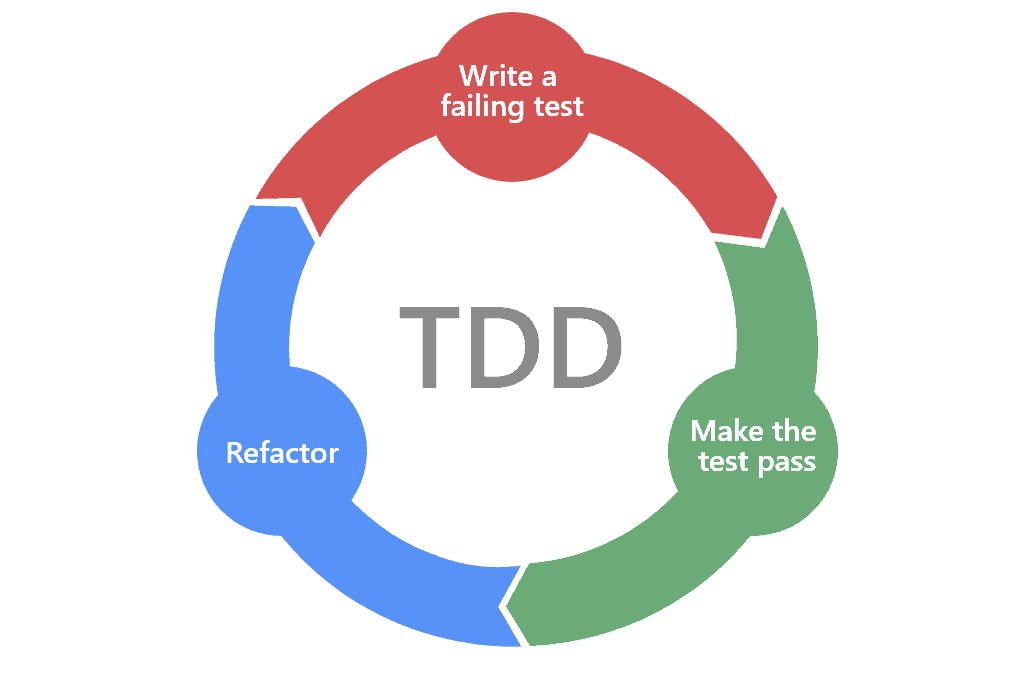
\includegraphics[width=0.70\textwidth]{figuras/ciclo-tdd.png}
  \caption{Ciclo do desenvolvimento guiado por testes: escrever um teste que
    falha, implementar o necessário para fazê-lo passar e refatorar.
    Fonte: \href{https://marsner.com/wp-content/uploads/test-driven-development-TDD.png}{Marsner}.}
  \label{fig:ciclo-tdd}
\end{figure}

Inspirado nas abordagens estudadas, este trabalho compara 
dois pipelines de geração de código a partir dos mesmos
requisitos em linguagem natural. Na geração direta, denominada baseline, o
agente produz a implementação sem receber resultados de testes durante a
geração. No pipeline baseado em TDD, um agente gera testes e outro implementa
e corrige o código com base nesses testes, até que passem ou que se atinja um
limite de execução. A comparação busca verificar se essa organização produz
código mais correto nos casos avaliados. Os testes gerados pelo próprio pipeline
são parte do processo de implementação; a avaliação usa testes externos a ele.

% % vamo fazer aqui um pedacinho sobre corretude. talvez ainda dentro do capitulo da introducao, pois estamos definindo as bases pro que vamos precisar mais adiante no TCC ainda. basicamente o que define um código como "correto" ou "melhor" que outro, pra gente ter como base pra comparar nos dois pipelines depois
% % É importante definirmos o que consideramos correto ou não, com base em testes de software determinísticos. Existem critérios que são obviamente determinísticos, tal qual o resultado de uma soma (sei la bota um snippet pytest bem idiota simples de testar uma funcao de soma). alguns, ainda determinísticos, mas difícieis de distignuir (bota um exemplo mais complexo, tipo teste de coisas em paralelo/threads nao sei). já outros são completamente subjetivos e é um problema difícil decidir se o resultado é correto ou não (bota um exemplo de teste subjetivo, pensei no exemplo de teste que o CUA pega na etapa dos experimentos com formularios, fala aquilo mas ainda nao fala do CUA).

\section{Corretude e critérios de avaliação}
\label{sec:corretude}

\subsubsection{Corretude}

Como observa \citet[seção~2.1]{dijkstra1969structured}, testes podem revelar a
presença de defeitos, mas sua execução sem falhas não demonstra a ausência deles.

Neste trabalho, a corretude funcional é entendida como o atendimento ao
comportamento especificado nos requisitos.

\subsubsection{Critérios objetivos}

Um teste automatizado verifica uma
parte desse comportamento ao executar uma ação e comparar o resultado observado
com o esperado. Por exemplo, se uma função deve somar dois inteiros, o
Programa~\ref{lst:teste-soma} verifica uma entrada cujo resultado é conhecido.

\begin{lstlisting}[language=Python,caption={Teste de uma função de soma.},label={lst:teste-soma}]
from calculadora import soma


def test_soma():
    assert soma(6, 7) == 13
\end{lstlisting}

Esse teste verifica apenas o caso escolhido. Uma implementação que devolvesse
sempre o valor 13 também passaria nele, embora descumprisse o requisito para
outras entradas. Assim, a aprovação em um conjunto de testes fornece evidência
sobre os casos exercitados, sem demonstrar a corretude geral da implementação.

Há também requisitos objetivos cuja verificação exige controlar condições de
execução mais complexas. Considere um contador iniciado em zero que recebe dois
incrementos concorrentes.

\begin{lstlisting}[language=Python,caption={Teste que força a perda de um incremento concorrente.},label={lst:teste-contador}]
from threading import Barrier, Thread


def test_incrementos_concorrentes():
    contador = 0
    barreira = Barrier(2)

    def incrementar():
        nonlocal contador
        valor = contador
        barreira.wait()
        contador = valor + 1

    threads = [Thread(target=incrementar) for _ in range(2)]
    for thread in threads:
        thread.start()
    for thread in threads:
        thread.join()

    assert contador == 2
\end{lstlisting}

No Programa~\ref{lst:teste-contador}, a barreira faz as duas threads aguardarem
até que ambas tenham lido o contador. As duas leem zero e escrevem 1, fazendo
a asserção falhar.
Se ambos os incrementos devem ser contabilizados, o valor final
esperado é 2. Uma implementação incorreta pode perder um incremento quando as
operações se intercalam, mas produzir o resultado esperado em outra execução.
O critério de aceitação continua objetivo; a dificuldade está em exercitar a
intercalação que revela a falha. Nesse caso, repetir uma execução sem controlar
a ordem das operações pode deixar o defeito sem detecção.

\subsubsection{Critérios subjetivos}

A qualidade de uma interface inclui ainda aspectos que exigem julgamento.
Em um formulário, conferir se os dados preenchidos são preservados ao trocar
de aba permite comparar valores antes e depois da ação. Já avaliar se o
espaçamento separa adequadamente os blocos de campos ou se a organização visual
facilita a leitura exige interpretar a apresentação no contexto de uso.
Esses julgamentos podem ser orientados por critérios explícitos, embora não se
reduzam à comparação de um valor com uma resposta única.

O formulário da Figura~\ref{fig:formulario-identidade-usp} ilustra essa dificuldade:
a presença do logotipo e das cores da USP pode ser verificada isoladamente,
mas avaliar se sua combinação caracteriza a identidade visual da instituição
exige definir o que se espera da apresentação como um todo.

\begin{figure}[htp]
  \centering
  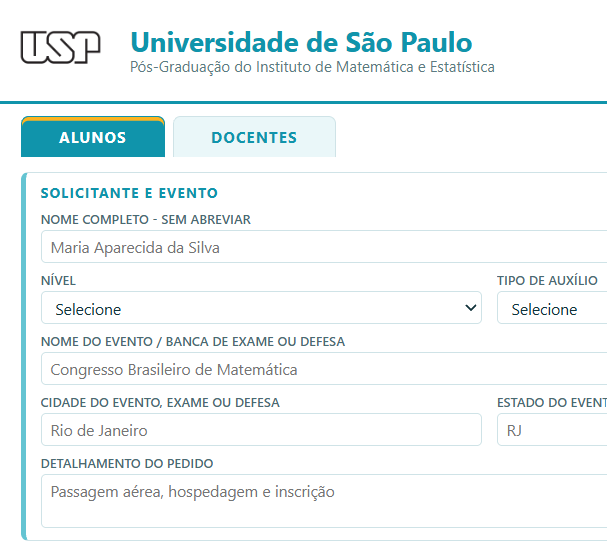
\includegraphics[width=0.80\textwidth]{figuras/formulario-torneio-cego.png}
  \caption{Como pedir para um teste automatizado verificar que essa interface
    segue a identidade visual da USP? Recorte do formulário da run44
    (DeepSeek, baseline), vencedora do torneio cego. Fonte: elaboração própria.}
  \label{fig:formulario-identidade-usp}
\end{figure}

Na comparação entre implementações, atender a mais casos de teste indica melhor
desempenho nos comportamentos avaliados. A clareza da interface requer uma
avaliação própria, com seus critérios e justificativas. Essas duas dimensões
permitem delimitar em que sentido uma implementação é considerada melhor que outra.

\chapter{Harness}
\label{cap:harness}
% Vamos primeiro entender como funciona um harness. Um harness é, segundo o https://github.com/HKUDS/OpenHarness,
% a infraestrutura completa que envolve uma LLM para permitir que ela haja sobre um ambiente.
% Nesse TCC (em algum lugar dos diarios acho eu defini isso bonitinho, acho que no blog/2026-08-19-harness.md), definimos o ambiente principal como um diretório num sistema de arquivos, operado via shell (linha de comando).
% (baixar e descrever e botar essa imagem aqui, guardar num diretorio padronizado do TCC, seila onde: https://cdn.prod.website-files.com/65c81e88c254bb0f97633a71/69cba9b378fbdcbc9db3067e_image.png)
% 
% O Harness é responsável por manter um loop agêntico. Tal qual um chat bot convencional, o harness recebe uma entrada do usuário (prompt), envia para a LLM, recebe a resposta da LLM e envia de volta para o usuário. 
% A diferença é que, no caso do harness, as respostas da LLM podem vir em formato de ferramentas (tool calls), que são comandos que o harness pode executar no ambiente.
% 
% No nosso caso, o harness recebe uma entrada num formato específico (alvo.toml e criterios.toml + pasta com arquivos arbitrários)
% essa entrada é o que padronizamos para ambos pipelines (Baseline e TDD).
% (Mostrar um exemplo mínimo dos arquivos .toml)
% 
% a CLI do harness opera com os seguintes argumentos:
% (listar argumentos e explicar cada um deles em uma frase simples)

Um harness é a infraestrutura que envolve um modelo de linguagem para permitir
que ele atue como agente em um ambiente \citep{openharness}. O harness recebe a
entrada do usuário, monta o contexto enviado ao modelo e processa sua resposta.
Essa resposta pode conter chamadas de ferramentas (\emph{tool calls}), que
solicitam ações como ler um arquivo ou executar um comando. O harness executa as
ações e devolve os resultados ao modelo, que pode usá-los para decidir o próximo
passo. Esse ciclo constitui o laço agêntico.

A Figura~\ref{fig:harness-generico} apresenta componentes de um harness genérico.
Além da execução de ações, o diagrama inclui o fornecimento de contexto, o
controle do fluxo, a persistência de informações e a observação dos resultados.
As próximas subseções detalham a arquitetura do harness desenvolvido neste TCC,
a partir de sua entrada e de sua interface de linha de comando.

\begin{figure}[htp]
  \centering
  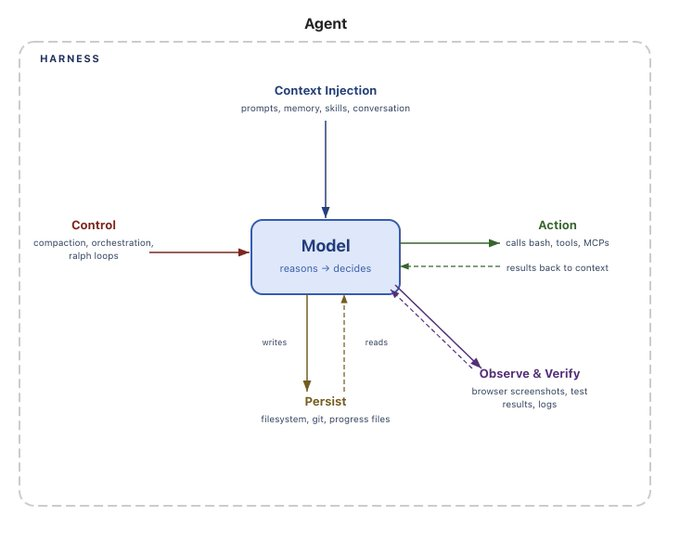
\includegraphics[width=0.70\textwidth]{figuras/harness-generico.png}
  \caption{Componentes de um harness genérico: contexto, controle, ações,
    persistência e verificação. Fonte: \citet{trivedy2026harness}.}
  \label{fig:harness-generico}
\end{figure}

\section{Arquitetura do harness}
\label{sec:arquitetura-harness}

O ambiente principal do harness deste TCC é um diretório no sistema de arquivos,
onde ficam os arquivos do projeto gerado. O harness grava esses arquivos e
executa os comandos definidos para iniciar a aplicação e realizar os testes.
Os grupos baseline e TDD usam o mesmo formato de entrada.

\subsection{Entrada}
\label{subsec:entrada-harness}

Na configuração com avaliação por Cypress e CUA, cada caso de uso ocupa um
diretório com três arquivos: \texttt{requisito.md},
que descreve, em linguagem natural, o software a gerar; \texttt{alvo.toml}, que define sua configuração
de execução; e \texttt{criterios.toml}, que reúne os critérios de aceitação para
a avaliação final. O diretório também pode conter pastas com imagens, fontes ou
outros arquivos de apoio. Essas pastas são copiadas para o projeto antes da
geração, exceto aquelas cujo nome começa com ponto ou sublinhado.

O arquivo \texttt{alvo.toml} declara os comandos da aplicação e dos testes,
a versão do Python, os pacotes disponíveis, os modelos usados em cada papel e
os limites de passos, custo e tempo por etapa de geração. No comando da
aplicação, \texttt{\{porta\}} é substituído por uma porta livre. O
Programa~\ref{lst:alvo} apresenta a configuração do caso de uso do formulário
de auxílio financeiro.

\begin{lstlisting}[language={},caption={Exemplo de \texttt{alvo.toml}.},label={lst:alvo}]
[comandos]
app = "uvicorn app:app --host 127.0.0.1 --port {porta}"
teste = "pytest -q --tb=short"
teste_frontend = "cypress run --project . --config-file _harness/cypress.config.js --browser chrome"

[dependencias]
python = "3.11"
pacotes = ["pytest==9.1.1", "fastapi[standard]==0.143.1"]

[modelos]
test_writer = "deepseek/deepseek-v4.1-flash"
coder = "deepseek/deepseek-v4.1-flash"
cua = "anthropic/claude-opus-5"

[orcamento]
passos = 50
custo_usd = 2.0
tempo_s = 1800
\end{lstlisting}

Em \texttt{criterios.toml}, cada bloco \texttt{[[criterios]]} contém um
identificador, o tipo do critério, a ação a realizar e o resultado esperado.
O tipo \texttt{deterministico} encaminha o critério para testes de interface com
Cypress; o tipo \texttt{subjetivo} o encaminha para avaliação pelo CUA.
Os testes de interface dependem também do comando \texttt{teste\_frontend}
em \texttt{alvo.toml}.
O Programa~\ref{lst:criterios} mostra um critério do mesmo caso de uso.

\begin{lstlisting}[language={},float=htp,breakatwhitespace=true,caption={Exemplo de critério em \texttt{criterios.toml}.},label={lst:criterios}]
[[criterios]]
identificador = "C3"
tipo = "deterministico"
acao = '''
Abrir a página inicial, conferir que os campos `NÍVEL` e `TIPO DE AUXÍLIO` estão na tela,
e então clicar na aba `DOCENTES`.
'''
resultado_esperado = '''
A aba `DOCENTES` fica ativa e o formulário mostrado não tem mais os campos `NÍVEL` nem
`TIPO DE AUXÍLIO` - eles existem só na aba `ALUNOS`. Os outros campos continuam lá.
'''
\end{lstlisting}

\subsection{Interface de linha de comando}
\label{subsec:cli-harness}

A CLI oferece os subcomandos \texttt{run}, para gerar um projeto, e
\texttt{avaliar}, para executar a avaliação final de um projeto já gerado.
A partir do diretório \texttt{demos/}, as chamadas têm a seguinte forma,
com argumentos opcionais entre colchetes:

\begin{lstlisting}[language={},numbers=none]
uv run python -m harness.cli run destino [requisito] \
    [--yes] [--direto] [--sem-cua]
uv run python -m harness.cli avaliar projeto requisito
\end{lstlisting}

\begin{itemize}
  \item \texttt{destino}: pasta na qual \texttt{run} cria um novo diretório para
    o projeto, com nome composto pelo caso de uso, grupo e data e hora da execução.
  \item \texttt{requisito}: caminho do diretório do caso de uso; se omitido em
    \texttt{run}, a CLI solicita um nome, copia o caso de uso de exemplo e abre
    seus arquivos no editor.
  \item \verb|--yes|: dispensa a aprovação humana ao final de cada etapa de
    geração.
  \item \verb|--direto|: seleciona o grupo baseline; sem essa opção, a geração
    segue o pipeline TDD.
  \item \verb|--sem-cua|: adia toda a avaliação final, incluindo Cypress e CUA,
    que pode ser executada depois com \texttt{avaliar}.
  \item \texttt{projeto}: diretório já gerado sobre o qual \texttt{avaliar}
    executa a avaliação e regrava \texttt{AVALIACAO.log} em
    \texttt{\_harness/}.
  \item \verb|-h| ou \verb|--help|: exibe a ajuda da CLI ou do subcomando escolhido.
\end{itemize}


\subsection{Extensões para o experimento do PreJanus}

O experimento do PreJanus-back reutiliza o harness com uma entrada e uma avaliação
próprias. Nesse experimento, a geração termina sem executar Cypress ou CUA; em seguida,
um gabarito de testes independente avalia o código gerado. Portanto,
\texttt{criterios.toml} não é necessário nesse fluxo. Os resultados do gabarito
são registrados em \texttt{GABARITO.json} e não retornam ao agente para corrigir
a implementação.

Além de baseline e TDD, o experimento inclui o grupo \emph{rework}, que gera uma
implementação do zero a partir de testes visíveis e contratos, sem receber o
código original nem o documento de requisitos do sistema. No TDD original,
os testes gerados ficam congelados durante a implementação; no rework, os
testes fornecidos também ficam congelados. A variante exploratória
\texttt{tdd-revisao} permite ao agente de implementação alterar os testes
autorais, preservando versões e diferenças para análise. Essas modalidades são
selecionadas pela interface específica do experimento, e não por novas opções da
CLI geral:

\begin{lstlisting}[language={},numbers=none]
uv run python -m caronte.piloto_v3 \\
    [baseline|tdd|rework|tdd-revisao]
\end{lstlisting}

\backmatter
\pagestyle{backmatter}
\printbibliography[title=\refname, heading=bibintoc]
\end{document}
